\subsubseccion{Distribuci\'on Beta}
\label{Sssec:MP:Beta}

Se denota $X  \sim \beta(a,b)$ \ con  \ $(a,b) \in \Rset_+^{* \,  2}$ \ llamados
{\em parametros de forma}.  Las caracter\'isticas son:

\begin{caracteristicas}
%
Dominio de definici\'on & $\X = [0 \; 1]$\\[2mm]
\hline
%
Parametros & $(a,b) \in \Rset_+^{* \, 2}$ (forma)\\[2mm]
\hline
%
Densidad   de    probabilidad   &   $\displaystyle    p_X(x)   =   \frac{x^{a-1}
(1-x)^{b-1}}{B(a,b)}$\\[2mm]
\hline
%
Promedio & $\displaystyle m_X = \frac{a}{a+b}$\\[2mm]
\hline
%
Varianza &  $\displaystyle \sigma_X^2  = \frac{a b}{(a  + b)^2  (a + b  + 1)}$\\[2mm]
\hline
%
\modif{Sesgo} & $\displaystyle \gamma_X = \frac{2 \, (b - a) \sqrt{a + b + 1}}{( a
+ b + 2) \sqrt{a b}}$\\[2mm]
\hline
%
Curtosis por exceso & $\displaystyle \widebar{\kappa}_X = \frac{6 \, \left( (a - b)^2 (a + b + 1) - a
b (a  + b  + 2)  \right)}{a \, b  \left( a  + b  + 2 \right)  \left( a  + b  + 3
\right)}$\\[2mm]
\hline
%
Generadora de momentos & $\displaystyle M_X(u)  = \hypgeom{1}{1}\left( a , a + b
\, ; \, u \right)$ \ para \ $u \in \Cset$\\[2mm]
\hline
%
Funci\'on     caracter\'istica     &     $\displaystyle     \Phi_X(\omega)     =
\hypgeom{1}{1}\left( a , a + b \, ; \, \imath \omega \right)$
\end{caracteristicas}

Su densidad de probabilidad y funci\'on de repartici\'on son representadas en la
figura Fig.~\ref{Fig:MP:Beta} para varios $a$ \ y \ $b$.
%
\begin{figure}[h!]
\begin{center} 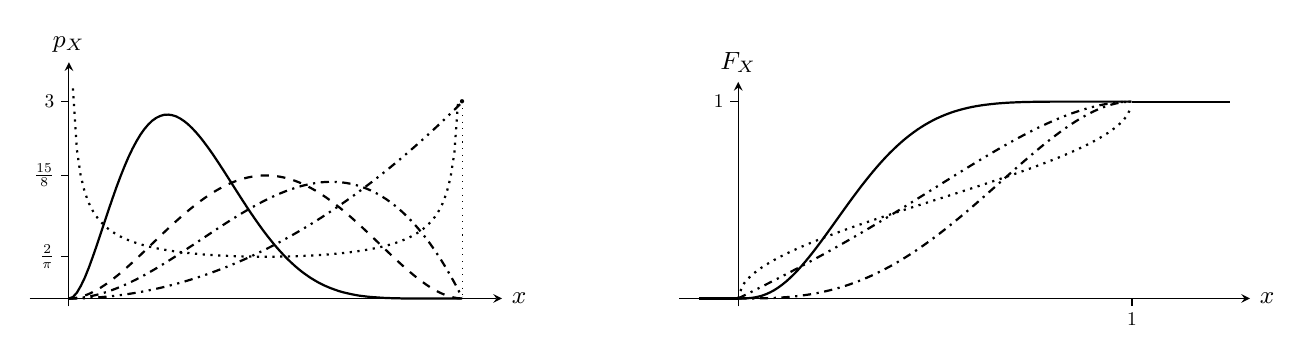
\begin{tikzpicture}%[scale=.9]
\shorthandoff{>}
%
\pgfmathsetmacro{\sx}{5};% x-scaling
\pgfmathsetmacro{\b}{7};% tercera eleccion de (3,beta)
\pgfmathsetmacro{\r}{.05};% radius arc non continuity F_X
%\pgfmathsetmacro{\mb}{max(2,\b*(\b+1)*((\b-1)^(\b-1))/((\b-2)^\b))};% maximo pdf para alpha = 2
\pgfmathsetmacro{\mb}{max(3,2*\b*(\b+2)/(\b+1)*(((\b-1)/(\b+1))^(\b-1))};% maximo pdf para alpha = 3
%
%
% densidad
\begin{scope}
%
%\pgfmathsetmacro{\sy}{2.5*((\b/(\b-1))^(\b-1))/(\b+1)};% y-scaling 
\pgfmathsetmacro{\sy}{2.5/\mb};% y-scaling
\draw[>=stealth,->] (-.5,0)--({\sx+.5},0) node[right]{\small $x$};
\draw[>=stealth,->] (0,-.1)--(0,3) node[above]{\small $p_X$};
%
%\draw[thick] (-.25,0)--(0,0);\draw (\r,\r) arc (90:270:\r);
%\draw[thick] (\sx,0)--({\sx+.25},0);\draw ({\sx-\r},{-\r}) arc (-90:90:\r);
% (a,b) = ( .5 , .5 )
\draw[thick,dotted,domain=.01:.99,samples=100] plot ({\x*\sx},{\sy*1/(pi*sqrt(\x*(1-\x)))});
% (a,b) = ( 2 , 1 )
%\draw[thick,dashed,domain=0:1,samples=100] plot ({\x*\sx},{\sy*2*\x}) node[scale=.4]{$\bullet$};
%\draw[dotted] (\sx,{2*\sy})--(\sx,0);
% (a,b) = ( 3 , 1 )
\draw[thick,dash dot dot,domain=0:1,samples=100] plot ({\x*\sx},{\sy*3*(\x^2)}) node[scale=.4]{$\bullet$};
\draw[dotted] (\sx,{3*\sy})--(\sx,0);
% (a,b) = ( 2 , 2 )
%\draw[thick,dash dot,domain=0:1,samples=100] plot ({\x*\sx},{\sy*6*\x*(1-\x)});
% (a,b) = ( 3 , 2 )
\draw[thick,dash dot,domain=0:1,samples=100] plot ({\x*\sx},{\sy*12*(\x^2)*(1-\x)});
% (a,b) = ( 3 , 3 )
\draw[thick,dashed,domain=0:1,samples=100] plot ({\x*\sx},{\sy*30*(\x^2)*((1-\x)^2)});
% (a,b) = ( 2 , b_3 )
%\draw[thick,domain=0:1,samples=100] plot ({\x*\sx},{\sy*\b*(\b+1)*\x*((1-\x)^(\b-1))});
% (a,b) = ( 3 , b_4 )
\draw[thick,domain=0:1,samples=100] plot ({\x*\sx},{\sy*.5*\b*(\b+1)*(\b+2)*(\x^2)*((1-\x)^(\b-1))});
%}
%
\draw (0,{\sy*2/pi})--(-.1,{\sy*2/pi}) node[left,scale=.7]{$\frac2\pi$};
\draw (0,{\sy*3})--(-.1,{\sy*3}) node[left,scale=.7]{$3$};
\draw (0,{\sy*15/8})--(-.1,{\sy*15/8}) node[left,scale=.7]{$\frac{15}{8}$};
%\draw (0,{\sy*1.5})--(-.1,{\sy*1.5}) node[left,scale=.7]{$\frac32$};
%\draw (0,{\sy*(\b+1)*((1-1/\b)^(\b-1))})--(-.1,{\sy*(\b+1)*((1-1/\b)^(\b-1))}) node[left,scale=.7]{$6 \left(\frac{4}{5} \right)^4$};
%\draw (\sx,0)--(\sx,-.1) node[below,scale=.7]{$1$};
%
\end{scope}
%
%
% reparticion
\begin{scope}[xshift=8.5cm]
%
\pgfmathsetmacro{\sy}{2.5};% y-scaling 
%
\draw[>=stealth,->] (-.75,0)--({\sx*1.25+.25},0) node[right]{\small $x$};
\draw[>=stealth,->] (0,-.1)--(0,{\sy+.25}) node[above]{\small $F_X$};
%
% cumulativa
\draw[thick] (-.5,0)--(0,0); \draw[thick] (\sx,\sy)--({\sx*1.25},\sy);
% (a,b) = ( .5 , .5 )
\draw[thick,dotted,domain=0:1,samples=100] plot ({\x*\sx},{\sy*(.5+asin(2*\x-1)/180)});
% (a,b) = ( 2 , 1 )
%\draw[thick,dashed,domain=0:1,samples=100] plot ({\x*\sx},{\sy*(1-(1+\x)*(1-\x))});
% (a,b) = ( 3 , 1 )
\draw[thick,dash dot dot,domain=0:1,samples=100] plot ({\x*\sx},{\sy*(1-(1+\x+\x^2)*((1-\x)^2))});
% (a,b) = ( 2 , 2 )
%\draw[thick,dash dot,domain=0:1,samples=100] plot ({\x*\sx},{\sy*(1-(1+2*\x)*((1-\x)^2))});
% (a,b) = ( 3 , 2 )
\draw[thick,dash dot,domain=0:1,samples=100] plot ({\x*\sx},{\sy*(1-(1+2*\x+3*\x^2)*((1-\x)^2))});
% (a,b) = ( 2 , b_3 )
%\draw[thick,domain=0:1,samples=100] plot ({\x*\sx},{\sy*(1-(1+\b*\x)*((1-\x)^\b))});
% (a,b) = ( 3 , b_4 )
\draw[thick,domain=0:1,samples=100] plot ({\x*\sx},{\sy*(1-(1+\b*\x+.5*\b*(\b+1)*\x^2)*((1-\x)^\b))});
%
\draw (0,\sy)--(-.1,\sy) node[left,scale=.7]{$1$};
\draw (\sx,0)--(\sx,-.1) node[below,scale=.7]{$1$};
\end{scope}
%
\end{tikzpicture} \end{center}
%
\leyenda{Ilustraci\'on de una densidad de  probabilidad beta (a), y la funci\'on
de  repartici\'on asociada (b).   $(a,b) =  (0.5 \,  , \,  0.5)$ (linea
punteada), $(3 \, , \, 1)$ (linea  mixta doble punteada), $(3 \, , \, 2)$ (linea
mixta), $(3 \, , \, 3)$ (linea
guionada), $(3 \, , \, 7)$ (linea llena).}
\label{Fig:MP:Beta}
\end{figure}

Nota que se recupera la  ley uniforme sobre \ $[0 \; 1]$ \  para \ $a = b =
1$. Se conoce la ley de $ 2 \, \beta\left( \frac12 , \frac12 \right) - 1$ \ como
{\em ley arcseno}.

Variables beta  tienen tambi\'en unas propiedades notables.  Primero, por cambio
de variables, se demuestra el lema siguiente:
%
\begin{lema}[Reflexividad]
\label{Lem:MP:ReflexividadBeta}
%
  Sea \ $X \, \sim \, \beta(a,b)$. Entonces
  %
  \[
  1-X \, \sim \, \beta(b,a)
  \]
  %
\end{lema}
%
\begin{lema}[V\'inculo con la ley gamma]
\label{Lem:MP:VinculoBetaGamma}
%
  Sea  \   $X  \,  \sim  \,   \G(a,c)$  \  e  \   $Y  \,  \sim   \,  \G(b,c)$  \
  independientes. Entonces
  %
  \[
  \frac{X}{X+Y} \, \sim \, \beta(a,b)
  \]
  %
  (independientemente  de $c$).   Adem\'as, $\frac{X}{X+Y}$  \ y  \ $X+Y$  \ son
  independientes.
\end{lema}
%
\begin{proof}
  La independencia de \ $c$ \ es obvia del hecho de que para cualquier $\theta >
  0, \: \theta^{-1} X \, \sim \, \G(a,\theta c)$ \ e \ $\theta^{-1} Y \, \sim \,
  \G(b,\theta  c)$,  la independencia  con  respeto  a \  $c$  \  viniendo de  \
  $\frac{\theta^{-1}     X}{\theta^{-1}     X     +     \theta^{-1}     Y}     =
  \frac{X}{X+Y}$.  Entonces, se  puede considerar  \ $c  = 1$  \ sin  perdida de
  generalidad. Ahora, sea la transformaci\'on
  %
  \[
  \begin{array}{lccl}
    g\ : & \Rset_+^2 & \mapsto & [0 \; 1] \times \Rset_+\\[1.5mm]
    %
    & (x,y) & \to & (u,v) = \left( \frac{x}{x+y} \, , \, x+y \right)
  \end{array}
  \]
  %
  Entonces, la transformaci\'on inversa se escribe
  %
  \[
  g^{-1}(u,v) = \left( u v \, , \, (1-u) v \right)
  \]
  %
  de matriz Jacobiana
  %
  \[
  \Jac_{g^{-1}} = \begin{bmatrix} v & u \\[2mm] -v & 1-u \end{bmatrix}
  \]
  %
  Del          teorema          de          cambio         de          variables
  teorema~\ref{Teo:MP:TransformacionBiyectiva},      notando     que     $\left|
    \Jac_{g^{-1}} \right| =  v$ \ y de la  independencia de \ $X$ \ e  \ $Y$, se
  obtiene para el vector aleatorio \ $W = \begin{bmatrix} U & V \end{bmatrix}^t$
  \ la densidad de probabilidad
  %
  \begin{eqnarray*}
    p_W(u,v) & = & p_X( u v ) \, p_Y( (1-u) v ) \, v\\[2mm]
    %
    & = & \frac{\left( u v \right)^{a-1} \, e^{- u v}}{\Gamma(a)} \times
    \frac{\left( (1-u) v \right)^{b-1} \, e^{- (1-u) v}}{\Gamma(b)} \times v\\[2mm]
    %
    & = & \frac{u^{a-1} (1-u)^{b-1}}{B(a,b)} \times \frac{v^{a+b-1} e^{-v}}{\Gamma(a+b)}
  \end{eqnarray*}
  %
  La  densidad se  obtiene por  marginalizaci\'on, \ie  integrando sobre  $v$ la
  densidad conjunta,  lo que  cierra la prueba  de la primera  parte.  Adem\'as,
  aparece claramente que \  $U$ \ y \ $V$ \ son  independientes (se factorisa la
  densidad de probabilidad).   Pasando, se recupera el hecho que  \ $X+Y \, \sim
  \, \G(a+b,1)$.
\end{proof}
%
\begin{lema}[Stabilidad por producto]
\label{Lem:StabilidadBeta}
%
  Sea  \  $X \,  \sim  \, \beta(a,b)$  \  e  \ $Y  \,  \sim  \, \beta(a+b,c)$  \
  independientes. Entonces
  %
  \[
  X Y \, \sim \, \beta(a,b+c)
  \]
  %
\end{lema}
%
\begin{proof}
  Sean \ $U  \, \sim \, \G(a,1)$, \ $V \,  \sim \, \G(b,1)$ \ y \  $W \, \sim \,
  \G(c,1)$   \   independientes  y   sean   \   $X   =  \frac{U}{U+V}$,   $Y   =
  \frac{U+V}{U+V+V}$  \ y  \ $Z  = U+V+W$.  Del lema  anterior \  $X \,  \sim \,
  \beta(a,b)$ \ y \ $Y \, \sim \, \beta(a+b,c)$. Sea la transformaci\'on
  %
  \[
  \begin{array}{lccl}
    g\ : & \Rset_+^3 & \mapsto & [0 \; 1]^2 \times \Rset_+\\[1.5mm]
    %
    & (u,v,w) & \to & (x,y,z) = \left( \frac{u}{u+v} \, , \, \frac{u+v}{u+v+w} \, , \, u+v+w \right)
  \end{array}
  \]
  %
  Entonces, la transformaci\'on inversa se escribe
  %
  \[
  g^{-1}(x,y,z) = \left( x y z \, , \, (1-x) y z \, , \, z (1-y) \right)
  \]
  %
  de matriz Jacobiana
  %
  \[
  \Jac_{g^{-1}} = \begin{bmatrix}
  %
    y z  &   x z   &   x y   \\[2mm]
  %
  - y z  & (1-x) z & (1-x) y \\[2mm]
  %
    0    &  - z    &  1-y
  %
  \end{bmatrix}
  \]
  %
  De      nuevo,      del      teorema      de     cambio      de      variables
  teorema~\ref{Teo:MP:TransformacionBiyectiva}, notando que $\left| \Jac_{g^{-1}}
  \right| = y  z^2$ \ y de la independencia  de \ $U, V, W$,  se obtiene para el
  vector aleatorio  \ $  T =  \begin{bmatrix} X &  Y &  Z \end{bmatrix}^t$  \ la
  densidad de probabilidad probabilidad
  %
  \begin{eqnarray*}
    p_T(x,y,z) & = & p_u( x y z ) \, p_V( (1-x) y z ) \, p_W( y (1-z) ) \, y z^2\\[2mm]
    %
    & = & \frac{\left( x y z \right)^{a-1} \, e^{- x y z}}{\Gamma(a)} \times
    \frac{\left( (1-x) y z \right)^{b-1} \, e^{- (1-x) y z}}{\Gamma(b)} \times
    \frac{\left( z (1-y) \right)^{c-1} \, e^{- z (1-y)}}{\Gamma(c)} \times y
    z^2\\[2mm]
    %
    & = & \frac{x^{a-1} (1-x)^{b-1}}{B(a,b)} \times \frac{y^{a+b-1}
      (1-y)^{c-1}}{B(a+b,c)} \times \frac{z^{a+b+c-1} e^{-z}}{\Gamma(a+b+c)}
  \end{eqnarray*}
  %
  Eso proba  que \  $X, \ Y$  \ y  $Z$ \ son  independientes (las  densidades se
  factorizan). Adem\'as,
  %
  \[
  X  Y =  \frac{U}{U+V} \times  \frac{U+V}{U+V+W} =  \frac{U}{U+V+W} \,  \sim \,
  \beta(a,b+c)
  \]
  %
  el      \'ultimo       resultado      como      consecuencia       de      los
  lemas~\ref{Lem:MP:VinculoBetaGamma}    y~\ref{Lem:MP:StabilidadGamma}.     Eso
  cierra la prueba.
\end{proof}

La distribuci\'on beta  aparece entre otros en problema  de inferencia Bayesiana
como   distribuci\'on   a   priori  conjugado~\footref{Foot:MP:BayesPrior}   del
parametro $p$ de la ley Binomial~\cite{Rob07}.

\SZ{Esta distribuci\'on aparece...}
% en  el conteo  de conteo  de  une repetici\'on  de una  experiencia de  maneja
% independiente hasta que  occure un evento de probabilidad  $p$; por ejemplo el
% n\'umero de tiro de un dado  equilibriado hasta que occurre un ``6'' sigue una
% ley geometrica de parametro $p = \frac16$.


La distribuci\'on beta  se generaliza al caso matriz-variada  $X$ definido sobre
$\X$  tal que $X$  y $I-X$  son en  $P_d^+(\Rset)$; se  denota \  $X \,  \sim \,
\beta_d(a,b)$ \ donde \ $(a,b) \in \Rset_+^{*  \, 2}$ y la densidad est dada por
$\displaystyle   p_X(x)    =   \frac{|x|^{a   -    \frac{d+1}{2}}   |I-x|^{b   -
    \frac{d+1}{2}}|}{B_p\left([a  \quad  b]^t\right)},  \quad (a,b)  \in  \left(
  \frac{d-1}{2} \; +\infty \right)^2$. Se refiera a~\cite[Cap.~5]{GupNag99} para
tener m\'as informaciones.